%%%%%%%%%%%%%%%%%%%%%%%%%%%%%%%%%%%%%%%%%%%%%%%%%%%%%
%%% Task 2 %%%%%%%%%%%%%%%%%%%%%%%%%%%%%%%%%%%%%%%%%%
%%%%%%%%%%%%%%%%%%%%%%%%%%%%%%%%%%%%%%%%%%%%%%%%%%%%%
\task{Working principle of a DC machine}
%%%%%%%%%%%%%%%%%%%%%%%%%%%%%%%%%%%%%%%%%%%%%%
\taskGerman{Wirkprinzipien der Gleichstrommaschine}
%%%%%%%%%%%%%%%%%%%%%%%%%%%%%%%%%%%%%%%%%%%%%%

\autoref{fig:dc_cross_section} shows a simplified DC machine cross section.
The symbols $\bullet$ and $\times$ indicate technical conductor current directions (out of / into the drawing plane).
Assume that the drawn field lines represent the complete air-gap field, i.e., no additional field lines exist
to the left and right of the shown field region. Thus, outside the depicted air-gap field region the flux density is assumed to be zero.

\begin{germanblock}
	Abbildung \autoref{fig:dc_cross_section} zeigt einen vereinfachten Querschnitt einer Gleichstrommaschine.
	Die Symbole $\bullet$ und $\times$ kennzeichnen die technischen Stromrichtungen der Leiter (aus / in die Bildebene).
	Nehmen Sie an, dass die eingezeichneten Feldlinien das vollständige Luftspaltfeld darstellen, d.\,h. es existieren keine weiteren
	Feldlinien rechts und links des dargestellten Feldbereichs. Außerhalb des dargestellten Luftspaltfeldes sei die Flussdichte somit Null.
\end{germanblock}

\begin{figure}[htb]
	\centering
	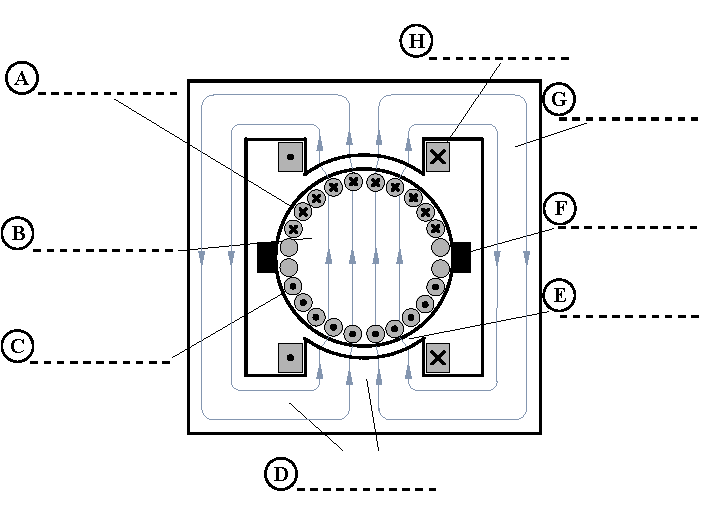
\includegraphics[width=0.7\linewidth]{fig/DC_machine_cross_section_without_text_labels.pdf}
	\caption{DC machine cross section with missing component labels.}
	\label{fig:dc_cross_section}
\end{figure}


For the calculations, assume a homogeneous and block-shaped air-gap flux density $\hat{B}_\delta$ within the pole coverage.
Use the data from \autoref{tab:DC_parameters} for the following calculations.

\begin{germanblock}
	Für die Berechnungen nehmen Sie eine homogene und blockförmige Luftspaltflussdichte $\hat{B}_\delta$ innerhalb der Polüberdeckung an. Verwenden Sie die Daten aus \autoref{tab:DC_parameters} für die folgenden Berechnungen.
\end{germanblock}

\begin{table}[htb]
	\centering
	\caption{Given DC machine parameters.}
	\label{tab:DC_parameters}
	\begin{tabular}{lll}
		\toprule
		Symbol             & Description                                        & Value                  \\
		\midrule
		$\hat{B}_\delta$   & Air-gap flux density (block-shaped)                & \SI{0.8}{\tesla}       \\
		$I_{\mathrm{c}}$   & Conductor current (per conductor)                  & \SI{218.75}{\ampere}   \\
		$l_z$              & Axial length                                       & \SI{0.25}{\meter}      \\
		$d_a$              & Armature diameter                                  & \SI{0.24}{\meter}      \\
		$p$                & Pole pairs                                         & \num{1}                \\
		$\alpha_p$         & Pole coverage factor                               & \num{0.65}             \\
		$n$                & Nominal rotational speed                           & \SI{2500}{\per\minute} \\
		$N_{\mathrm{act}}$ & Number of active conductors (4 forward + 4 return) & \num{8}                \\
		$a$                & Number of parallel armature paths                  & \num{1}                \\
		\bottomrule
	\end{tabular}
\end{table}



%%%%%%%%%%%%%%%%%%%%%%%%%%%%%%%%%%%%%%%%%%%%%%
\subtask{Add the missing component labels (A--H) in \autoref{fig:dc_cross_section}.}{2}
\subtaskGerman{Ergänzen Sie die fehlenden Bauteilbezeichnungen (A--H) in \autoref{fig:dc_cross_section}.}


\begin{solutionblock}
	The correct component labels are shown in \autoref{fig:dc_cross_section_solution}.
	\begin{solutionfigure}
		\centering
		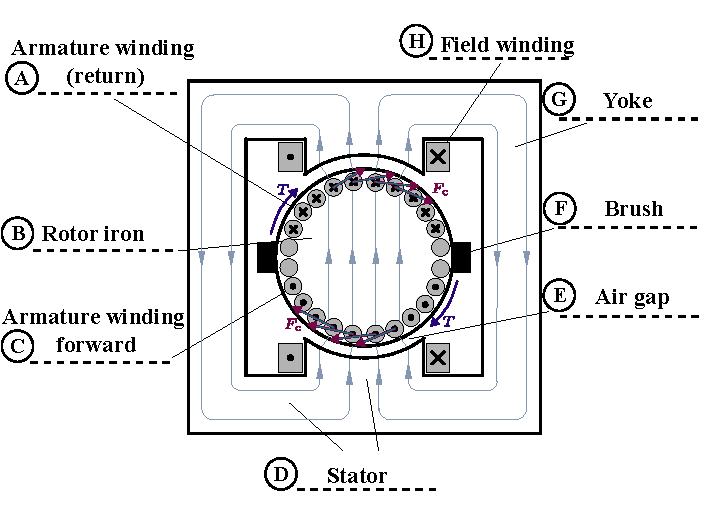
\includegraphics[width=0.7\linewidth]{fig/DC_machine_cross_section_with_solutions.pdf}
		\caption{DC machine cross section with component labels as well as torque and force indications.}
		\label{fig:dc_cross_section_solution}
	\end{solutionfigure}
\end{solutionblock}

%%%%%%%%%%%%%%%%%%%%%%%%%%%%%%%%%%%%%%%%%%%%%%
\subtask{In \autoref{fig:dc_cross_section}, draw the resulting Lorentz force on one exemplary forward conductor ($\bullet$) and one return conductor ($\times$). Also, indicate the resulting torque direction at the shaft.}{2}
\subtaskGerman{Zeichnen Sie in \autoref{fig:dc_cross_section} die resultierende Lorentzkraft an je einem beispielhaften Hinleiter ($\bullet$) und Rückleiter ($\times$) sowie die resultierende Drehmomentrichtung an der Welle ein.}


\begin{solutionblock}
	Apllying the Lorentz's force right hand law, the solution from \autoref{fig:dc_cross_section_solution} is obtained. As the force is acting on the armature conductors in a clockwise direction, the resulting torque is also in clockwise direction.
\end{solutionblock}

%%%%%%%%%%%%%%%%%%%%%%%%%%%%%%%%%%%%%%%%%%%%%%
\subtask{Calculate the Lorentz force $F_{\mathrm{c}}$ acting on one active armature conductor assuming a perpendicular field penetration through the air gap.}{1}
\subtaskGerman{Berechnen Sie die Lorentzkraft $F_{\mathrm{c}}$ auf einen aktiven Ankerleiter unter der Annahme einer senk\-rech\-ten Felddurchsetzung durch den Luftspalt.}

\begin{solutionblock}
	\[
		F_{\mathrm{c}}=\hat{B}_\delta\,l_z\,I_{\mathrm{c}}
		=\SI{0.8}{T}\cdot \SI{0.25}{m}\cdot \SI{218.75}{A}
		=\SI{43.75}{N}.
	\]
\end{solutionblock}

%%%%%%%%%%%%%%%%%%%%%%%%%%%%%%%%%%%%%%%%%%%%%%
\subtask{Calculate (i) the torque contribution $T_{\mathrm{c}}$ of one active conductor and (ii) the resulting shaft torque $T$ from all active conductors.}{2}
\subtaskGerman{Berechnen Sie (i) das Drehmoment eines aktiven Leiters $T_{\mathrm{c}}$ und (ii) das resultierende Drehmoment an der Welle $T$ aus allen aktiven Leitern.}



\begin{solutionblock}
	\[
		T_{\mathrm{c}} = F_{\mathrm{c}}\frac{d_a}{2}
		= \SI{43.75}{N}\cdot \frac{\SI{0.24}{m}}{2}
		= \SI{5.25}{N\,m}.
	\]
	With $N_{\mathrm{act}}=8$ active conductors (4 forward + 4 return),
	\[
		T = N_{\mathrm{act}}\,T_{\mathrm{c}} = 8\cdot \SI{5.25}{N\,m}=\SI{42}{N\,m}.
	\]
\end{solutionblock}

%%%%%%%%%%%%%%%%%%%%%%%%%%%%%%%%%%%%%%%%%%%%%%
\subtask{Compute the maximum flux linkage per armature coil $\hat{\phi}_\mathrm
		c$.}{2}
\subtaskGerman{Berechnen Sie die maximale Flussverkettung pro Leiterschleife.}

\begin{solutionblock}
	The pole pitch for $p=1$ is:
	\[
		\tau_p=\frac{\pi d_a}{2}=\frac{\pi\cdot \SI{0.24}{m}}{2}=\SI{0.377}{m}.
	\]
	The maximum flux linkage is given, when a conductor loop is covering the entire pole coverage area. Hence, the effective air-gap area is given by the pole coverage factor $\alpha_p$ times the pole pitch $\tau_p$ times the axial length $l_z$:
	\[
		A_\delta=\alpha_p\,\tau_p\,l_z=0.65\cdot \SI{0.377}{m}\cdot \SI{0.25}{m}=\SI{0.0613}{m^2}.
	\]
	The maximum flux linkage per conductor pair is then given by
	\[
		\hat{\phi}_\mathrm{c}=\hat{B}_\delta\,A_\delta
		=\SI{0.8}{T}\cdot \SI{0.0613}{m^2}
		=\SI{0.049}{\volt\second}.
	\]
\end{solutionblock}

%%%%%%%%%%%%%%%%%%%%%%%%%%%%%%%%%%%%%%%%%%%%%%
\subtask{Determine (i) the induced voltage magnitude $\hat{u}_{\mathrm{i,c}}$ per active conductor at the nominal speed and (ii) the total induced armature voltage magnitude $\hat{u}_{\mathrm{i}}$. For the latter assume that the voltage induction per conductor loop is roughly identical for all loops.}{3}

\subtaskGerman{Bestimmen Sie (i) die induzierte Spannungsamplitude $\hat{u}_{\mathrm{i,c}}$ pro aktivem Leiter bei der Nenndrehzahl und (ii) die gesamte induzierte Ankerspannungsamplitude $\hat{u}_{\mathrm{i}}$. Für Letzteres nehmen Sie an, dass die Spannungsinduktion pro Leiterschleife für alle Schleifen annähernd identisch ist.}


\begin{solutionblock}
	The nominal angular speed is given by:
	\[
		\omega=\frac{2\pi n}{60}=\frac{2\pi\cdot \SI{2500}{\per\minute}}{\SI{60}{\second\per\minute}}=\SI{261.8}{rad/s}.
	\]
	Due to the block-shaped flux density distribution, the flux linkage is linearly dependent on the rotor angle. Hence, for a constant speed, the induced voltage is given by the rotor angle derivative (angular speed) times the flux linkage:
	\[
		\hat{u}_{\mathrm{i,c}}=\omega \hat{\phi}_\mathrm{c}=\SI{261.8}{rad/s}\cdot \SI{0.049}{\volt\second}=\SI{12.8}{V}.
	\]
	The total induced voltage results from the four active conductor loops (4 forward + 4 return) in series connection, i.e., $N_{\mathrm{act}}/2=4$ conductor loops:
	\[
		\hat{u}_{\mathrm{i}} = \frac{N_{\mathrm{act}}}{2}\hat{u}_{\mathrm{i,c}} = 4\cdot \SI{12.8}{V}=\SI{51.2}{V}.
	\]
\end{solutionblock}